\section{\Large DISTURBANCES}
\subsection{Gravity Gradient}

The gravity gradient can generate a torque on our spacecraft while in orbit. The equations for the gravity gradient torque are below.
\begin{align*}
    I_x \dot{\omega_x} + (I_z - I_y) \omega_y \omega_z = 3 n^2 (I_z - I_y) c_y c_z \\
    I_y \dot{\omega_y} + (I_x - I_z) \omega_z \omega_x = 3 n^2 (I_x - I_z) c_z c_x \\
    I_z \dot{\omega_z} + (I_y - I_x) \omega_x \omega_y = 3 n^2 (I_y - I_x) c_x c_y \\
\end{align*}

In the above equation, $\Vec{c} = [c_x, c_y, c_z]^\intercal$ is the normalized direction of $\Vec{R}$.

The function \texttt{gravGrad} was developed to be used with \texttt{ode113} to propagate the Euler equations and kinematics with gravity gradient torques.

\lstinputlisting{src/gravGrad.m}
\lstinputlisting{src/gravGradTorque.m}

We can estimate the order of magnitude for gravity gradient torques using the following equation.
\begin{align*}
    \Vec{M} &= \frac{3 \mu}{a^3}
    \begin{bmatrix}
    (I_z - I_y) c_y c_z \\
    (I_x - I_z) c_z c_x \\
    (I_y - I_x) c_x c_y
    \end{bmatrix}
\end{align*}

The parameters used were the known moments of inertia ($I_x = \qty{7707}{}$, $I_y = \qty{14563}{}$, $I_z = \qty{18050}{\kilogram\cdot\meter^2}$), known values for Earth ($a = \qty{7125.49}{km}$, $\mu = \qty{398600}{\km^3\per\second^2}$), and an arbitrary $\Vec{c} = [\frac{1}{\sqrt{3}}, \frac{1}{\sqrt{3}}, \frac{1}{\sqrt{3}}]$. With these values, we arrive at:
\begin{align*}
    \Vec{M} &=
\qty[parse-numbers = false]{
    \begin{bmatrix}
    0.384174 \\
    1.13956 \\
    -0.755387
    \end{bmatrix}
    \cdot
    10^{-2}
}{\newton\meter}
\end{align*}

These values are in line with what we see in Figure \ref{fig:ps4_problem4e_torque}. We also expect gravity gradient torque to be zero, i.e., in equilibrium, when the principal axes are aligned with RTN and the angular velocity is the same as mean motion. Figures \ref{fig:ps4_problem4d_torque}, \ref{fig:ps4_problem4d_angvel} demonstrate zero torque when aligned with RTN frame and constant angular velocity. Simulating for longer periods reveals the torque error is periodically stable.

\begin{figure}[H]
\centering
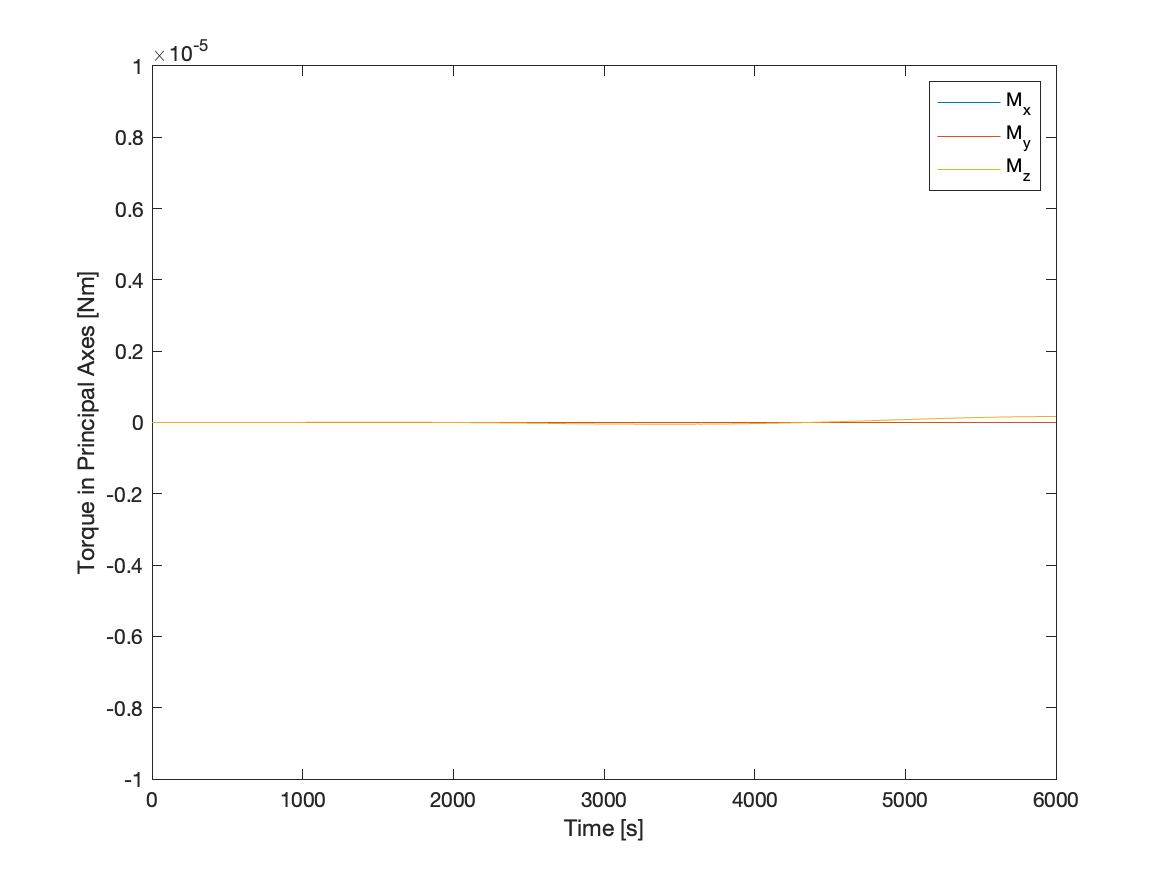
\includegraphics[scale=0.6]{Images/ps4_problem4d_torque.png}
\caption{Zero gravity gradient torque for satellite aligned with RTN frame}
\label{fig:ps4_problem4d_torque}
\end{figure}

\begin{figure}[H]
\centering
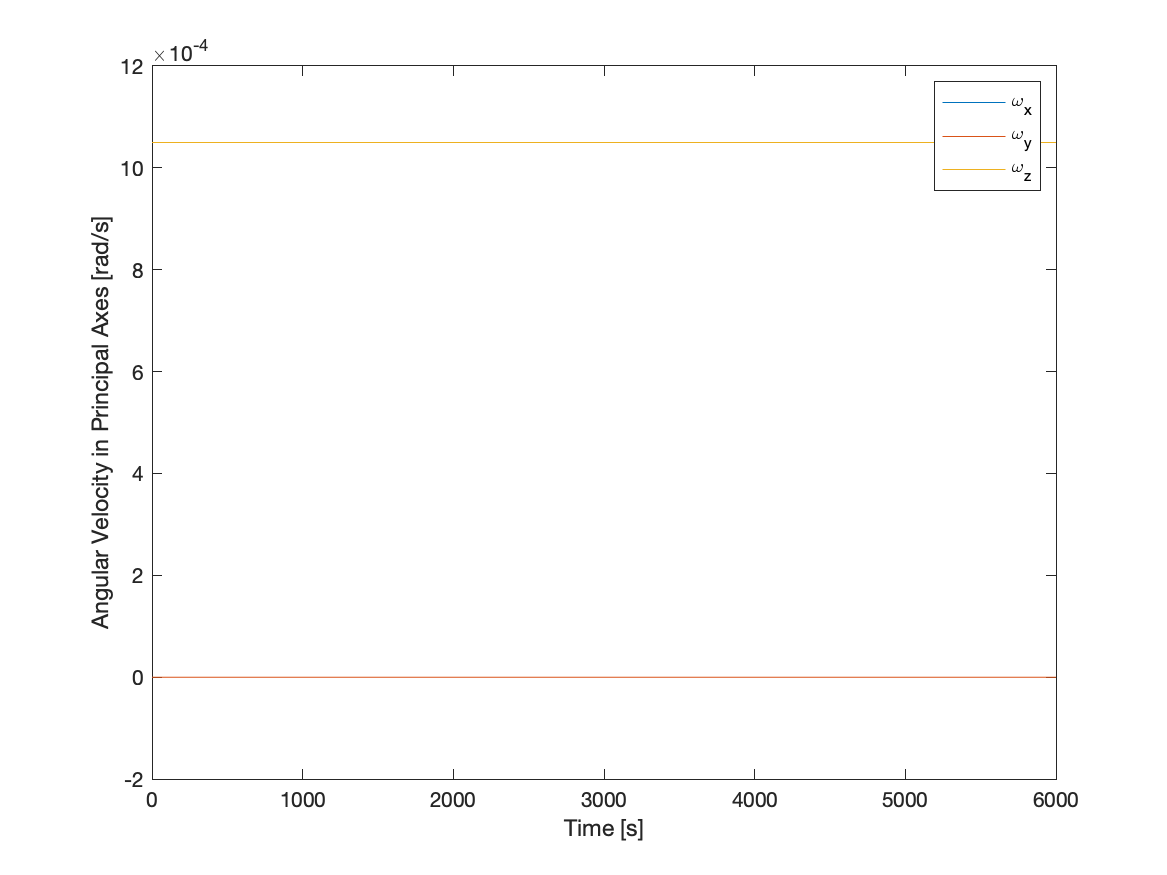
\includegraphics[scale=0.6]{Images/ps4_problem4d_angvel.png}
\caption{Angular velocity parallel to RTN normal equal to mean motion, all others zero}
\label{fig:ps4_problem4d_angvel}
\end{figure}

We align a permuted set of body axes for a different set of initial conditions, which will more closely resemble the orientation of the satellite when collecting science data.

\begin{figure}[H]
\centering
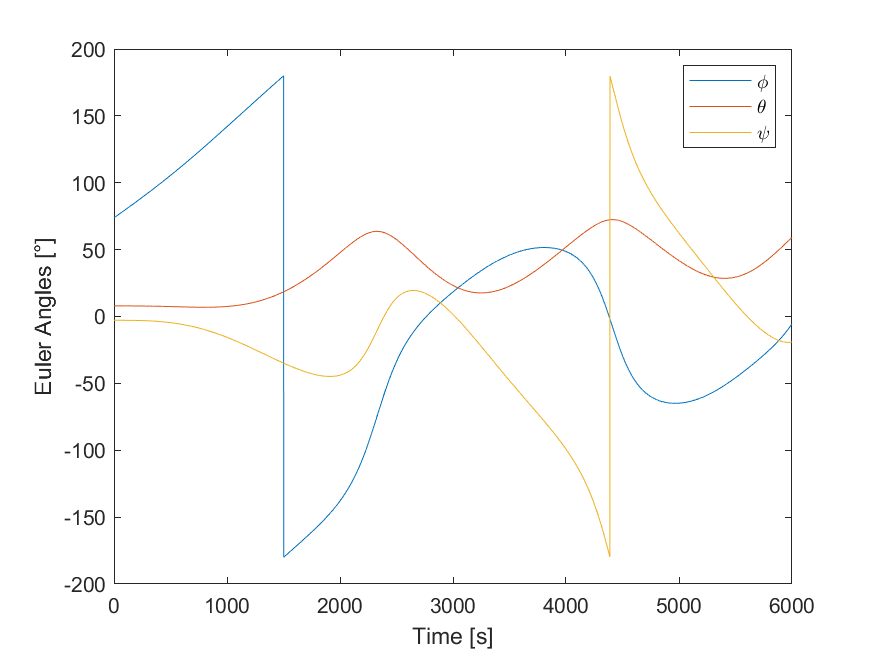
\includegraphics[scale=0.6]{Images/ps4_problem4e_angle.png}
\caption{Euler angles with gravity gradient for satellite with arbitrary initial conditions}
\label{fig:ps4_problem4e_angle}
\end{figure}

\begin{figure}[H]
\centering
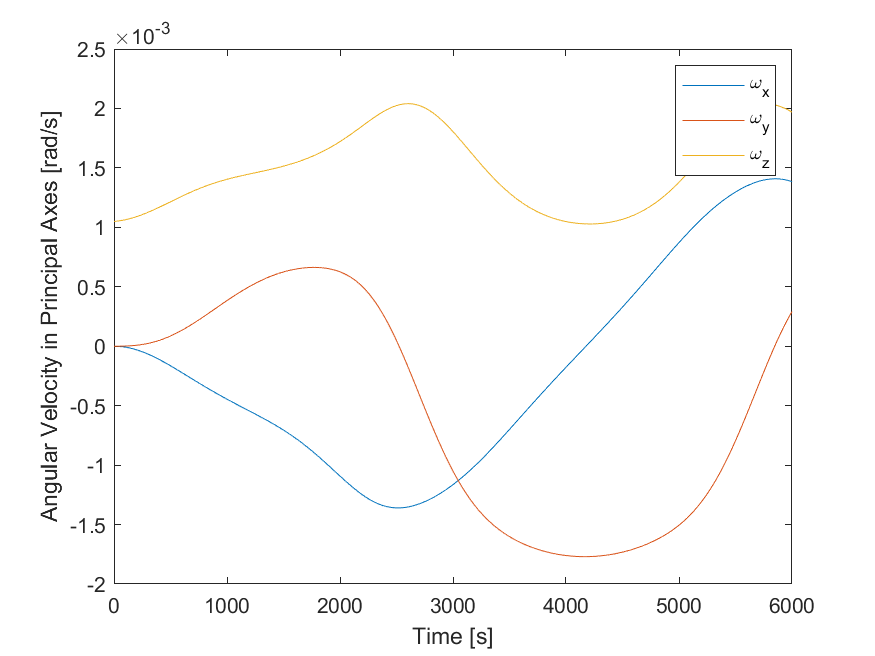
\includegraphics[scale=0.6]{Images/ps4_problem4e_angvel.png}
\caption{Angular velocity with gravity gradient for satellite with arbitrary initial conditions}
\label{fig:ps4_problem4e_angvel}
\end{figure}

The figures show that there is a noticeable effect of gravity gradient torque on the satellite, although the magnitude of the torque is low. This causes changes to our Euler angles throughout the orbit, meaning we will need a control system to stabilize and point our satellite in order to meet mission requirements.

\begin{figure}[H]
\centering
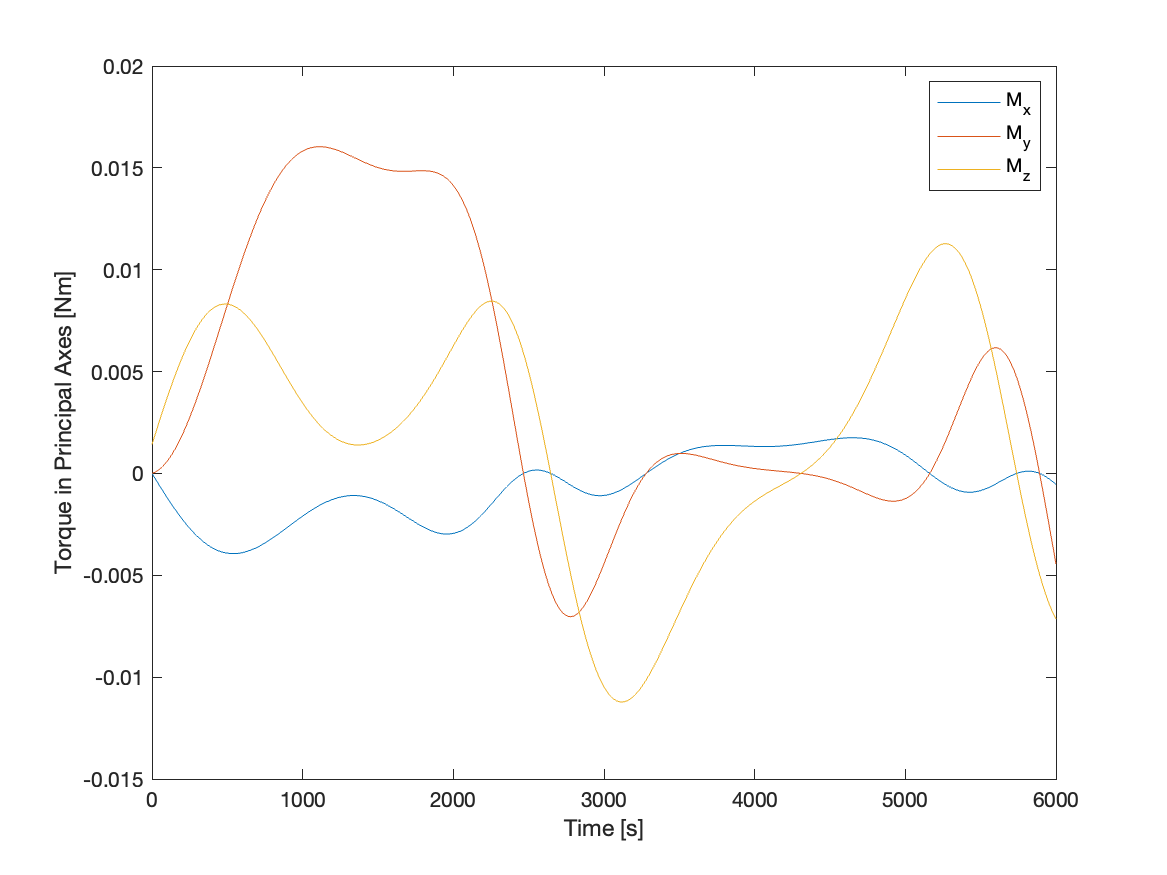
\includegraphics[scale=0.6]{Images/ps4_problem4e_torque.png}
\caption{Gravity gradient torques for satellite with arbitrary initial conditions}
\label{fig:ps4_problem4e_torque}
\end{figure}

\subsection{Stability, Gravity Gradient}

The following equations show the relationships for gravity gradient stability in terms of moments of inertia. The first inequality hold for when the pitch is stable, and the last two inequalites hold for when the roll and yaw are stable.
\begin{align*}
    k_N = \frac{I_T - I_R}{I_N}, \;\;\;\;\;
    k_T = \frac{I_N - I_R}{I_T}, \;\;\;\;\;
    k_R = \frac{I_N - I_T}{I_R} \\
    k_T > k_R, \;\;\;\;\;
    k_R k_T > 0, \;\;\;\;\;
    1 + 3 k_T + k_R k_T > 4 \sqrt{k_R k_T}
\end{align*}

We show the plot of stable and unstable motion under gravity gradient. When computing the coefficients using moments of inertia about the principal axes, we obtain the following plot. In this case, we investigate the stability for the satellite when it is rotated such that the spacecraft is oriented appropriately for SAR operations, that is, principal x-axis is anti-radial, principal y-axis is opposite of cross-track, and principal z-axis is opposite of along-track. However, this orientation is unstable, as shown below.

\begin{figure}[H]
\centering
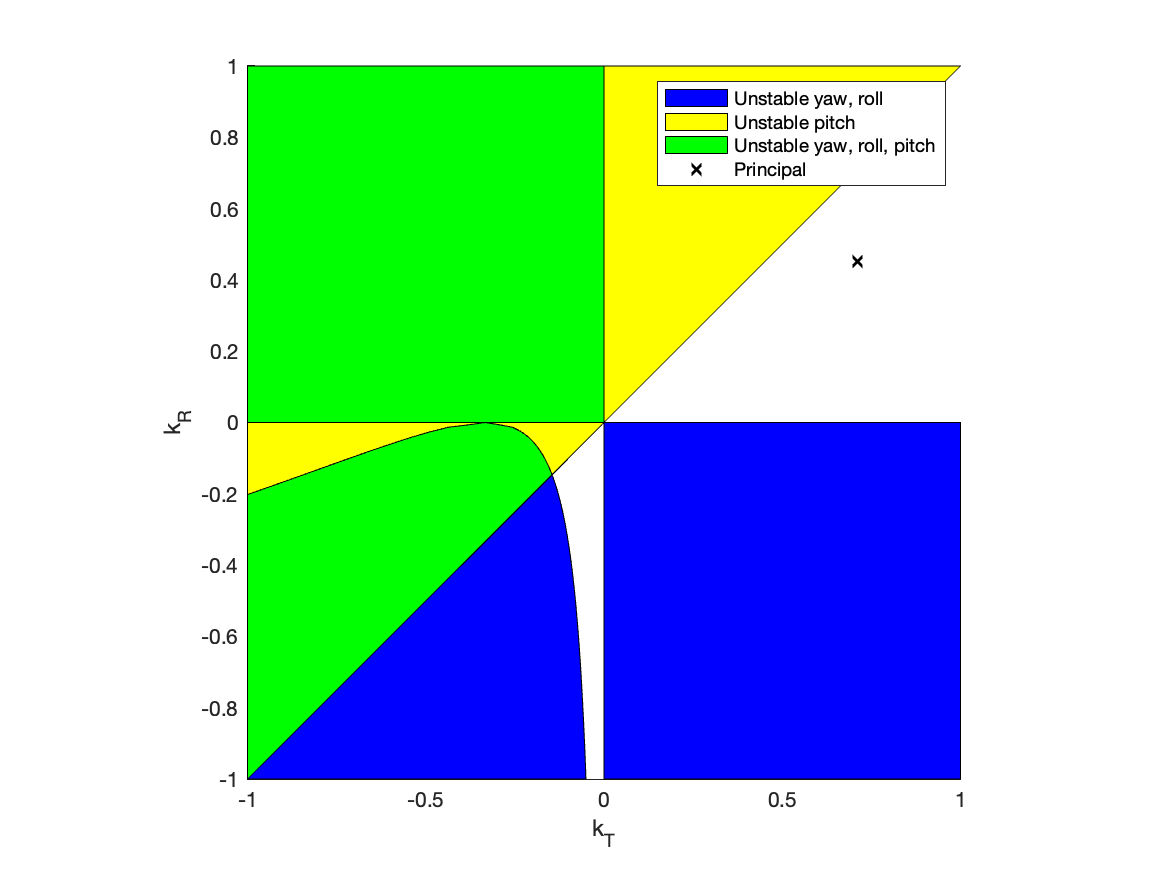
\includegraphics[scale=0.6]{Images/ps5_problem1a.png}
\caption{Stability for nominal axes}
\label{fig:ps5_problem1a}
\end{figure}

First, without perturbations, the satellite can maintain steady attitude, demonstrating that this chosen orientation is indeed an equilibrium.

\begin{figure}[H]
\centering
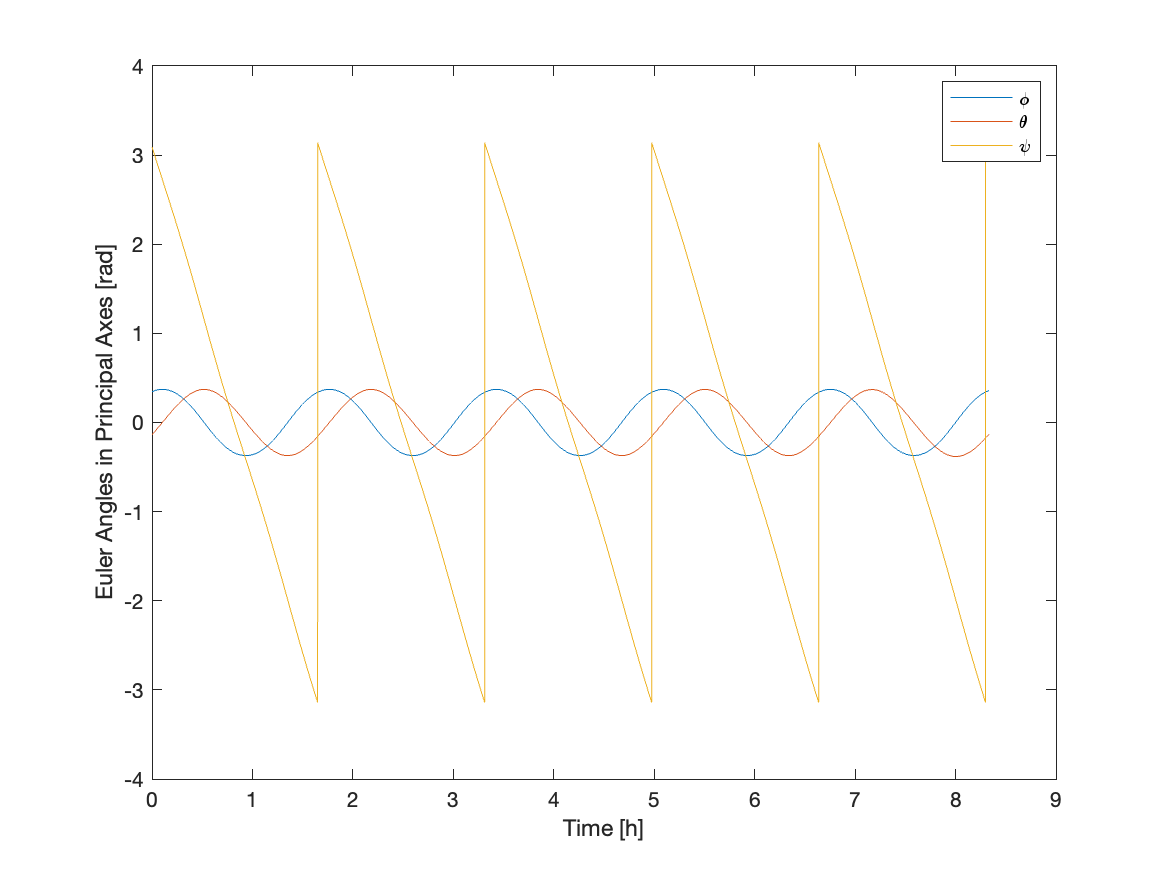
\includegraphics[scale=0.6]{Images/ps5_problem1b_angle_unperturbed.png}
\caption{Attitude evolution for unstable orientation without perturbations}
\label{fig:ps5_problem1b_angle_unperturbed}
\end{figure}

\begin{figure}[H]
\centering
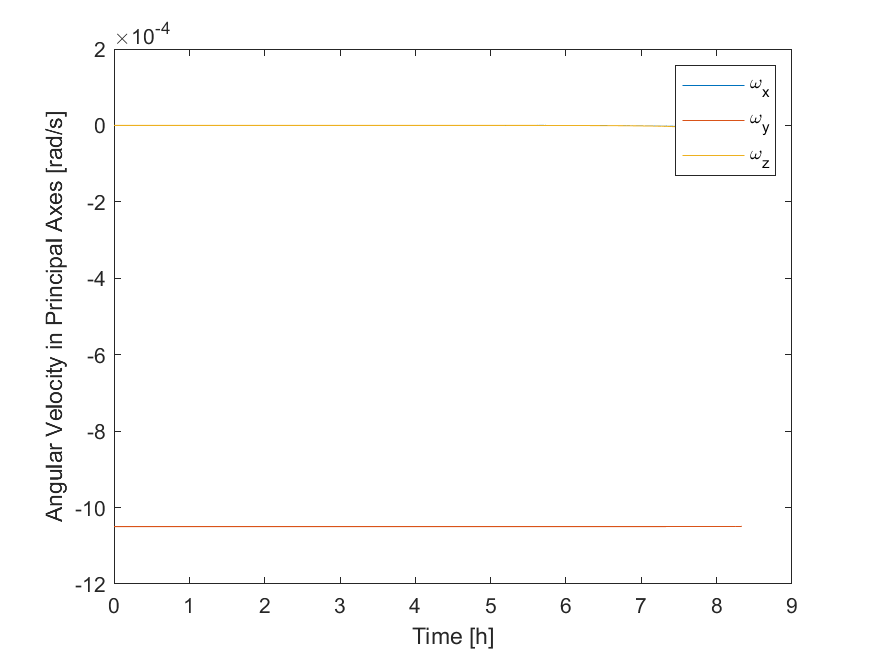
\includegraphics[scale=0.6]{Images/ps5_problem1b_angvel_unperturbed.png}
\caption{Angular velocity evolution for unstable orientation without perturbations}
\label{fig:ps5_problem1b_angvel_unperturbed}
\end{figure}

We expect unstable behavior for small perturbations. Previously, we have already shown that aligning principal axes with RTN produces stable behavior when there are no perturbations. Now, we will introduce small perturbations, causing the system to leave equilibrium and demonstrating that it is unstable.

\begin{figure}[H]
\centering
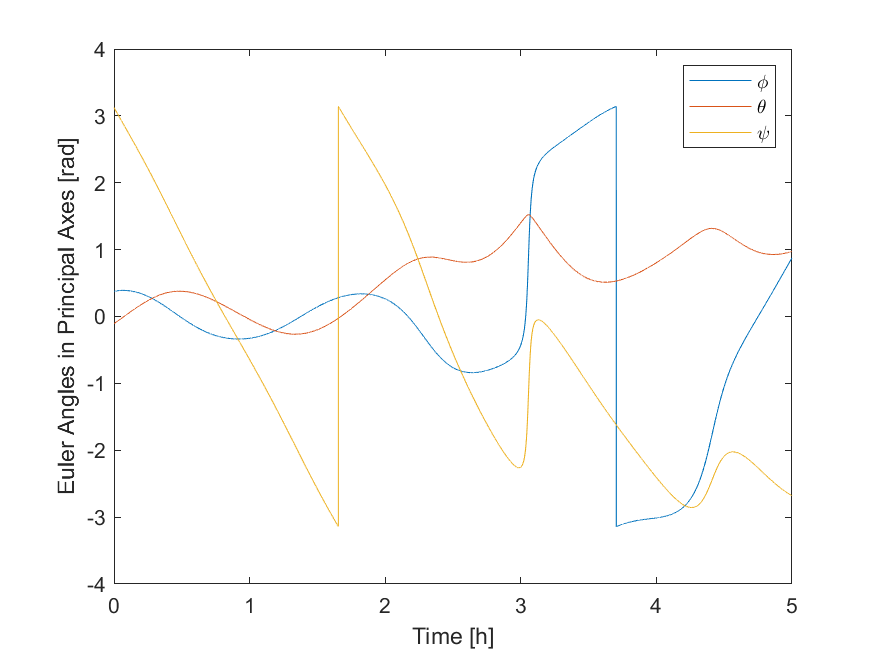
\includegraphics[scale=0.6]{Images/ps5_problem1b_angle.png}
\caption{Attitude evolution for unstable orientation with 1\% perturbations}
\label{fig:ps5_problem1b_angle}
\end{figure}

\begin{figure}[H]
\centering
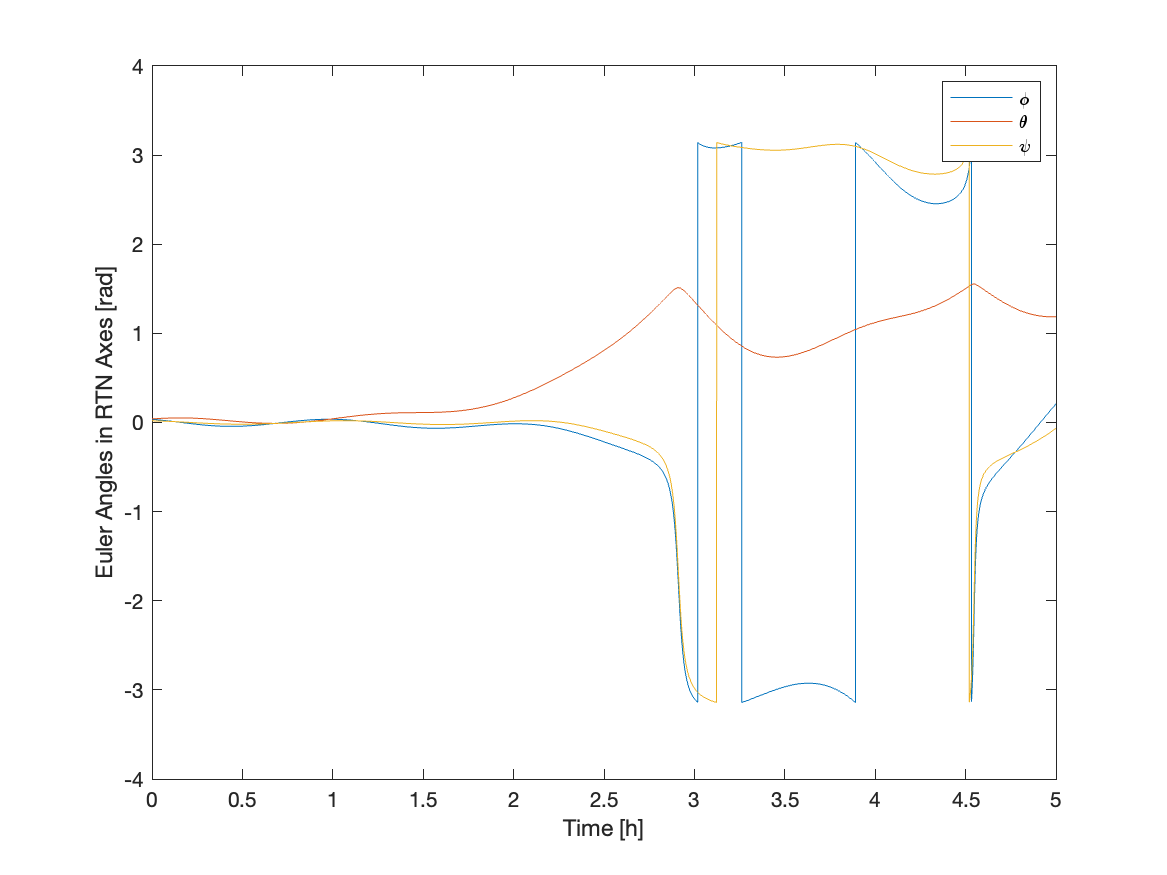
\includegraphics[scale=0.6]{Images/ps5_problem1b_angle_rtn.png}
\caption{Attitude evolution (relative to RTN) for unstable orientation with 1\% perturbations}
\label{fig:ps5_problem1b_angle_rtn}
\end{figure}

\begin{figure}[H]
\centering
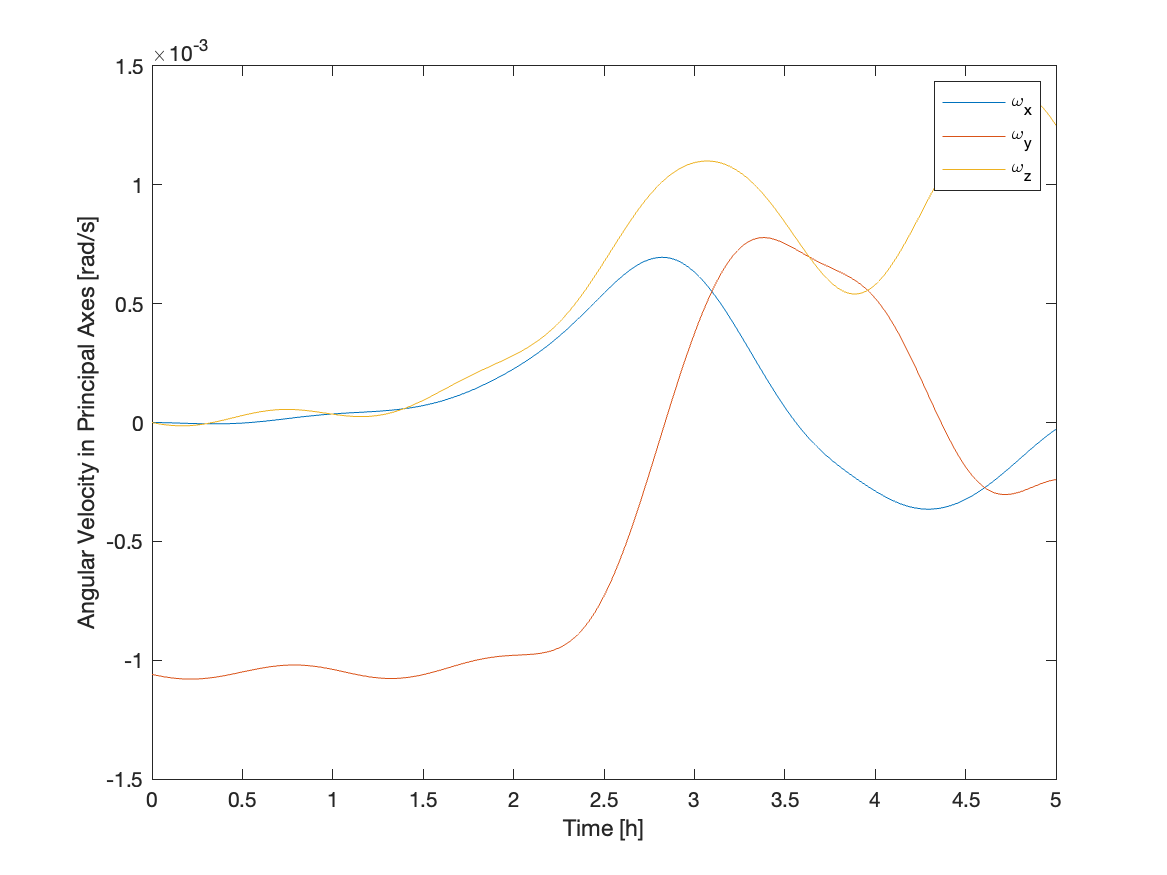
\includegraphics[scale=0.6]{Images/ps5_problem1b_angvel.png}
\caption{Angular velocity evolution for unstable orientation with 1\% perturbations}
\label{fig:ps5_problem1b_angvel}
\end{figure}

Now, we change the nominal attitude to generate stable motion due to gravity gradient torque. We will have to align the principal axes XYZ with RTN (respectively) to obtain a stable attitude motion.

\begin{figure}[H]
\centering
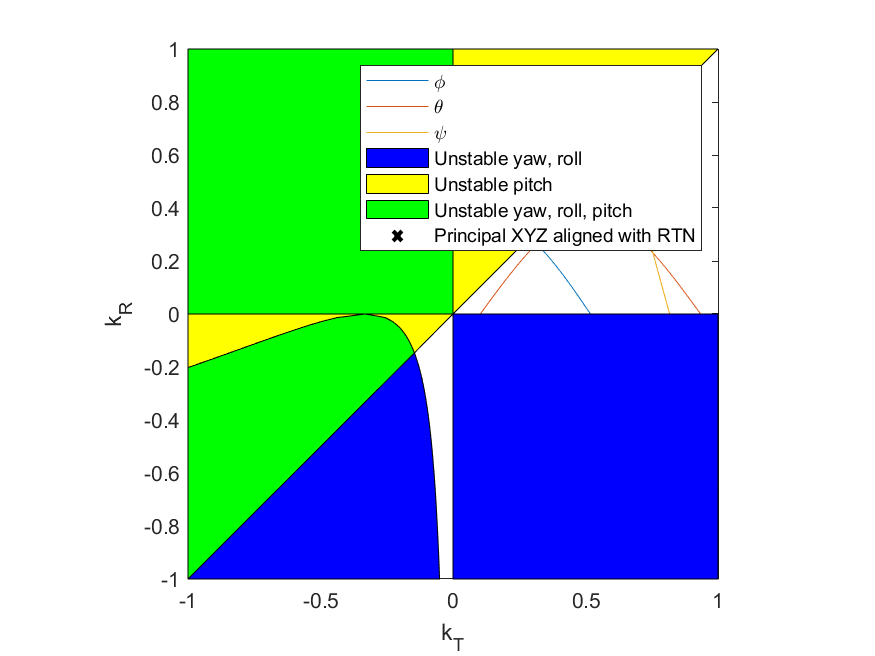
\includegraphics[scale=0.6]{Images/ps5_problem1c.png}
\caption{Stability for aligned principal axes}
\label{fig:ps5_problem1c}
\end{figure}

We expect stable behavior for small perturbations. Previously, we have already shown that aligning principal axes with RTN produces stable behavior when there are no perturbations. Now, we will introduce small perturbations.

\begin{figure}[H]
\centering
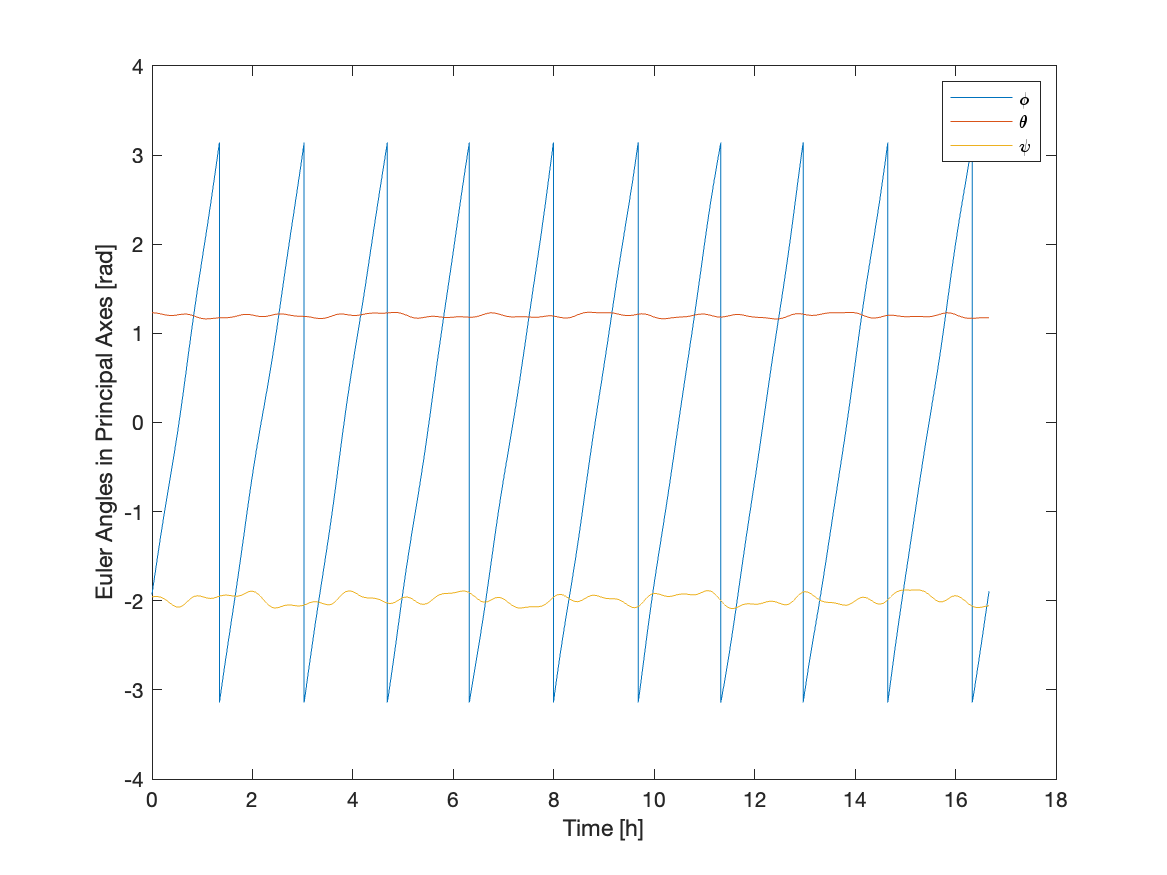
\includegraphics[scale=0.6]{Images/ps5_problem1c_angle.png}
\caption{Attitude evolution for stable orientation with 1\% perturbations}
\label{fig:ps5_problem1c_angle}
\end{figure}

\begin{figure}[H]
\centering
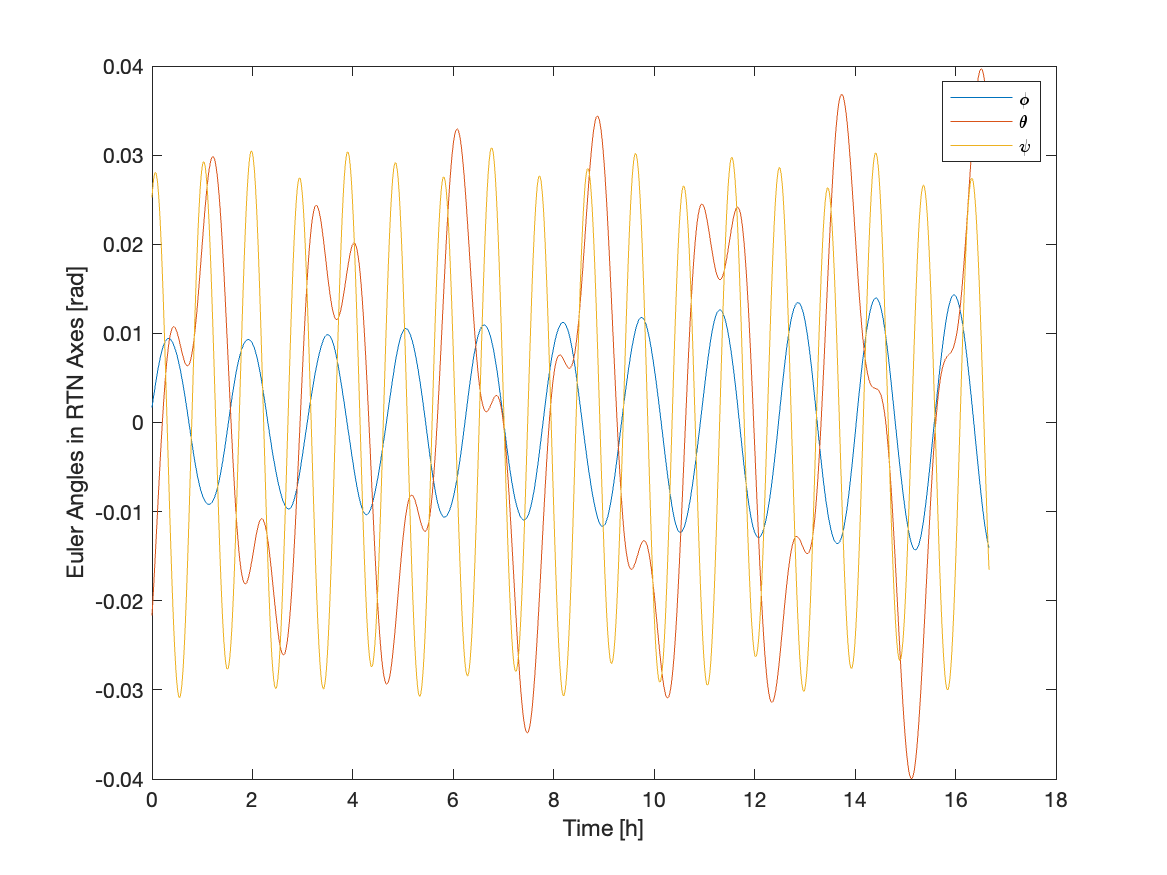
\includegraphics[scale=0.6]{Images/ps5_problem1c_angle_rtn.png}
\caption{Attitude evolution (relative to RTN) for stable orientation with 1\% perturbations}
\label{fig:ps5_problem1c_angle_rtn}
\end{figure}

\begin{figure}[H]
\centering
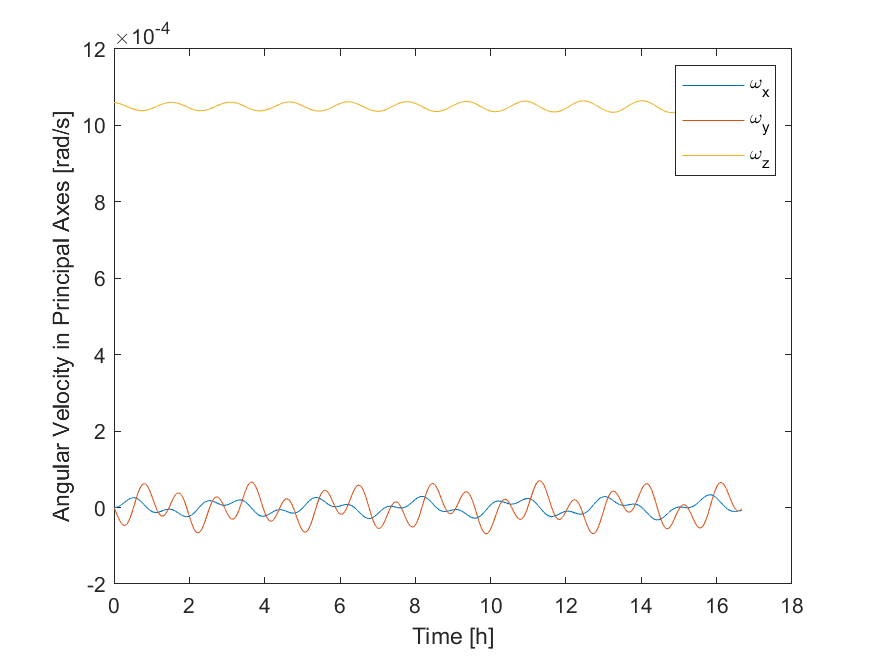
\includegraphics[scale=0.6]{Images/ps5_problem1c_angvel.png}
\caption{Angular velocity evolution for stable orientation with 1\% perturbations}
\label{fig:ps5_problem1c_angvel}
\end{figure}

As expected, our attitude motion (angular velocities and Euler angles) are periodically stable with a small perturbation in initial condition.

We cannot maintain this orientation if we want to properly point the radar antenna located at the top of the spacecraft, so it does not make sense to orient the satellite along principal axes for gravity gradient stability. Instead, we will likely require magnetorquers to offset angular momentum changes from environmental torques, including gravity gradient torques due to our unstable equilibrium.

\subsection{Magnetic Field}
In addition to gravity gradient torques, we modeled torque from magnetic field interactions, solar radiation pressure, and atmospheric drag.

The equation for the torque from the magnetic field interactions is shown below.
\begin{align*}
    \Vec{M}_{m} = \Vec{m}_{sat} \times \Vec{B}_{Earth}
\end{align*}

Since the satellite is operates in LEO, the spherical harmonic model up to n = 4 was used for maximum accuracy. This model is based on the geocentric distance ($R$), colatitude ($\theta$), and longitude ($\phi$). The model requires Gaussian coefficients ($g^{n,m}$, $h^{n,m}$) and Legendre functions ($P^{n,m}$) and their derivatives ($\frac{\delta P^{n,m} (\theta)}{\delta \theta}$), which are explained in more detail in Wertz \cite{Wertz}.
\begin{align*}
    B_R = \sum^{4}_{n=1} (\frac{R_{Earth}}{R})^{n+2} (n+1) \sum^{n}_{m=0}
    (g^{n,m} \cos{m \phi} + h^{n,m} \sin{m \phi}) P^{n,m}(\theta) \\
    B_{\theta} = - \sum^{4}_{n=1} (\frac{R_{Earth}}{R})^{n+2} \sum^{n}_{m=0}
    (g^{n,m} \cos{m \phi} + h^{n,m} \sin{m \phi}) \frac{\delta P^{n,m} (\theta)}{\delta \theta} \\
    B_{\phi} = - \frac{1}{\sin{\theta}} \sum^{4}_{n=1} (\frac{R_{Earth}}{R})^{n+2}
    \sum^{n}_{m=0} m (-g^{n,m} \sin{m \phi} + h^{n,m} \cos{m \phi}) P^{n,m}(\theta)
\end{align*}

\subsection{Solar Radiation Pressure}
The equations below define the solar radiation torque, where $C_S$ is the specular reflection coefficient, $C_d$ is the diffuse reflection coefficient, $\Vec{S}$ is the vector facing the Sun, and $e_i$ is 1 if the surface is illuminated and 0 otherwise. In implementation, we represent $e_i$ as a boolean tensor in tensor operations for fast computation.
\begin{align*}
    \Vec{M}_{S} = \sum^{n}_{i=1} \Vec{r}_{i} \times e_i \int_{S_i} d \Vec{f}_{total_{i}} \\
    d \Vec{f}_{total} = -P ((1-C_S) \hat{\Vec{S}} + 2 (C_S \cos{\theta} + \frac{1}{3} C_d) \cos{\theta} dA
\end{align*}

\subsection{Drag}
Finally, the equation below define the aerodynamic torque. Velocity is relative velocity of the spacecraft to the atmosphere, and we can compute the atmosphere's relative motion using a cross product of the position vector and Earth's rotational rate in ECI.
\begin{align*}
    d \Vec{f}_{aero} = - \frac{1}{2} C_D \rho V^2 (\hat{\Vec{V}} \cdot \hat{\Vec{N}}) \hat{\Vec{V}} dA
\end{align*}

Implementation of these disturbances in MATLAB code can be found in the appendix.

\subsection{Analysis}
For most torques, the worst-case estimated magnitudes were found by using existing properties of the spacecraft model. We use simplified equations (compared to those in the previous section) to estimate these, making assumptions for worst-case torques. However, the magnetic torque calculation assumes a model of the spacecraft's magnetic field as a single coil wrapped around the surface of the RIS and satellite bus. The estimated maximum values of each torque are listed in the table below.

\begin{table}[H]
\centering
\begin{tabular}{l|l} 

Magnetic Field & Estimated Maximum Value (N-m)  \\ 
\hline
$M_{gg}$          & 1.7093e-02                  \\ 
\hline
$M_{srp}$         & 1.8294e-02                  \\ 
\hline
$M_{drag}$        & 1.3682e-03                  \\ 
\hline
$M_{mag}$         & 1.3751e-10                  \\
\end{tabular}
\end{table}

In Figures \ref{fig:ps5_problem3_grav}, \ref{fig:ps5_problem3_drag}, \ref{fig:ps5_problem3_srp}, \ref{fig:ps5_problem3_mag}, we show the numerical simulation results for each type of disturbance based on the equations and code in the previous section. The numerical simulations indicate that the simulated results and estimated values are roughly within an order of magnitude for each type of disturbance torque shown.

\begin{figure}[H]
\centering
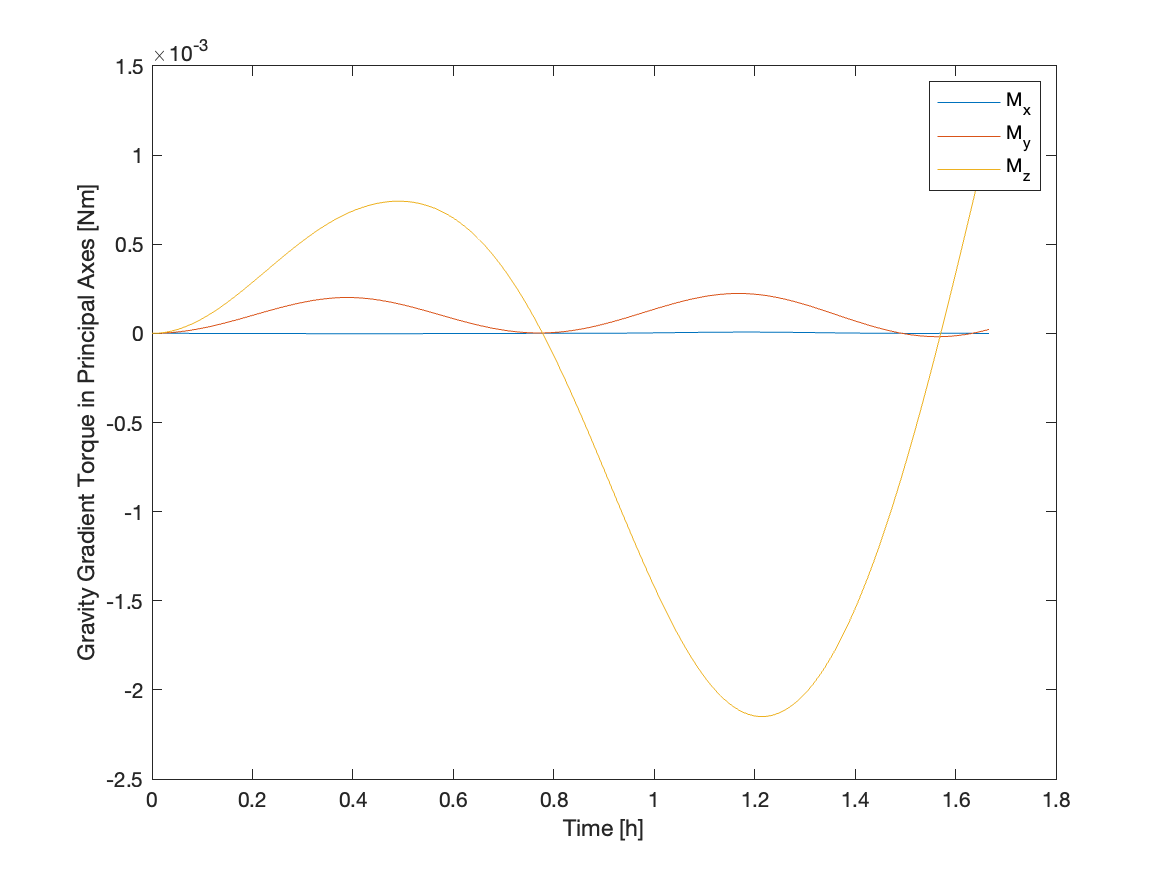
\includegraphics[scale=0.6]{Images/ps5_problem3_grav.png}
\caption{Numerical simulation of gravity gradient torques}
\label{fig:ps5_problem3_grav}
\end{figure}

\begin{figure}[H]
\centering
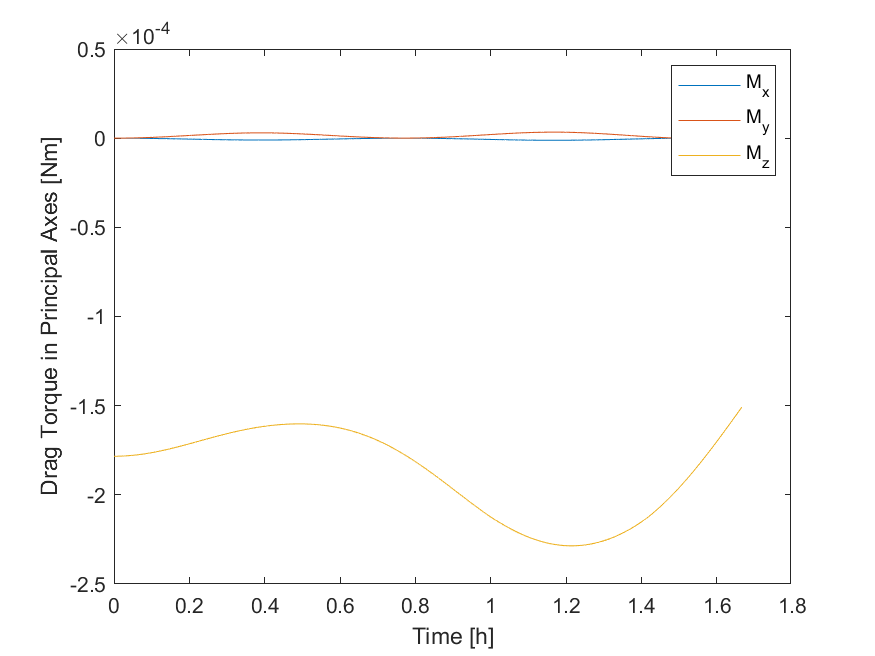
\includegraphics[scale=0.6]{Images/ps5_problem3_drag.png}
\caption{Numerical simulation of drag torques}
\label{fig:ps5_problem3_drag}
\end{figure}

\begin{figure}[H]
\centering
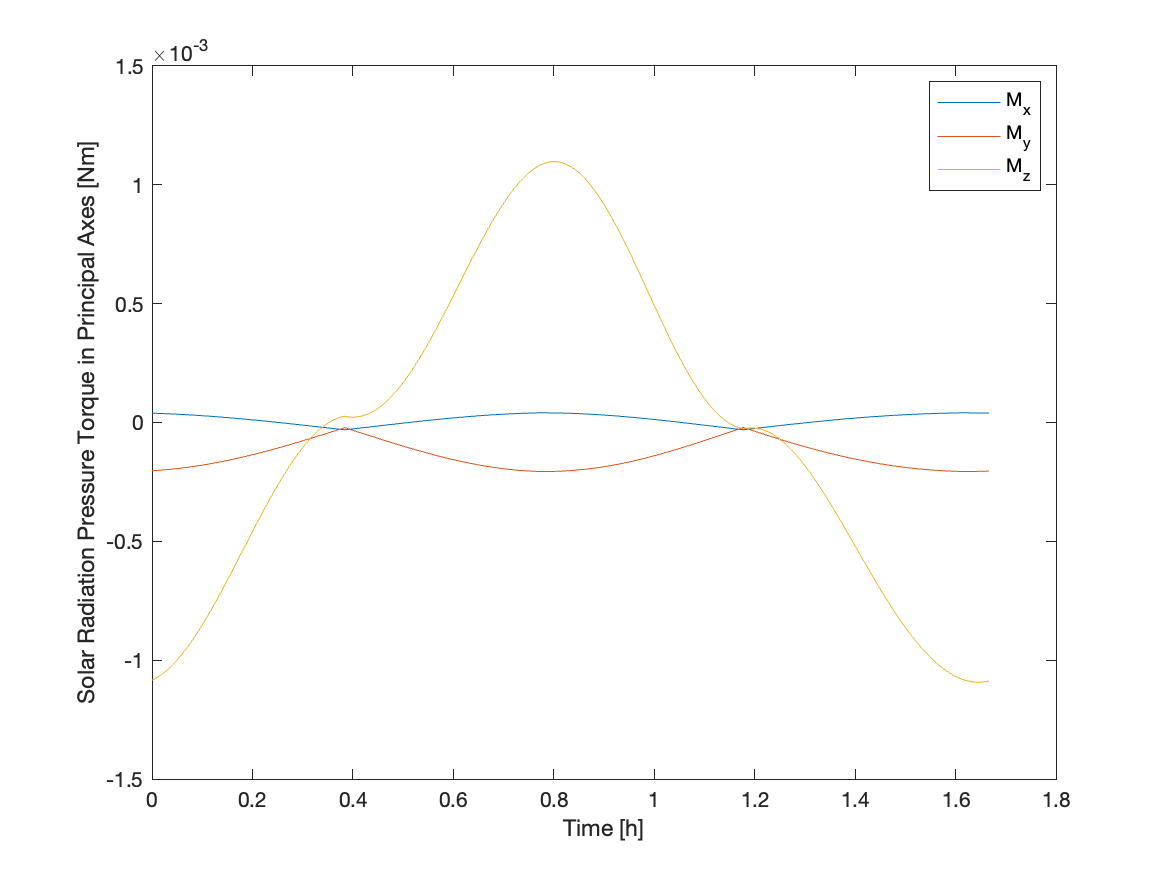
\includegraphics[scale=0.6]{Images/ps5_problem3_srp.png}
\caption{Numerical simulation of solar radiation pressure torques}
\label{fig:ps5_problem3_srp}
\end{figure}

\begin{figure}[H]
\centering
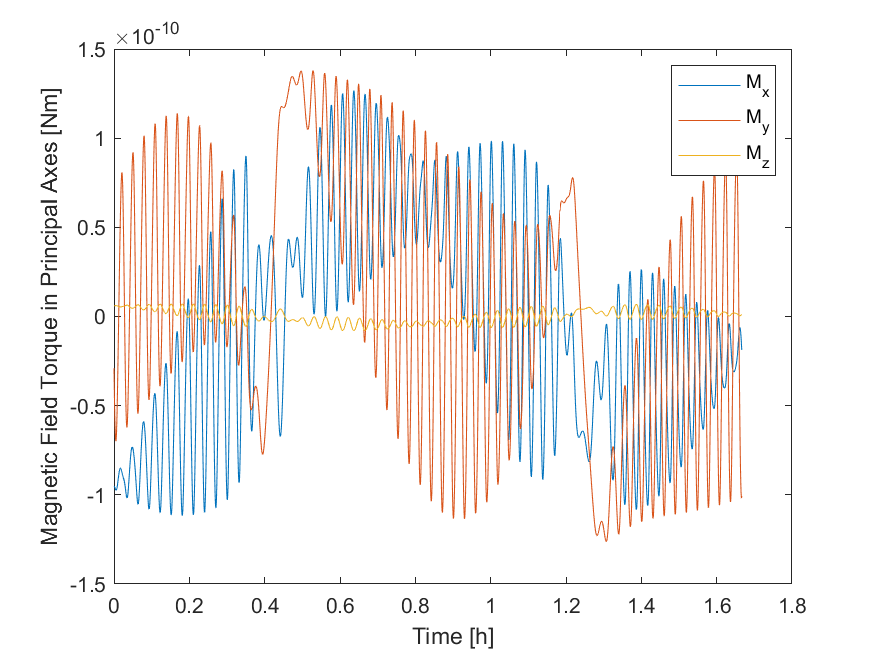
\includegraphics[scale=0.6]{Images/ps5_problem3_mag.png}
\caption{Numerical simulation of magnetic field torques}
\label{fig:ps5_problem3_mag}
\end{figure}

\begin{figure}[H]
\centering
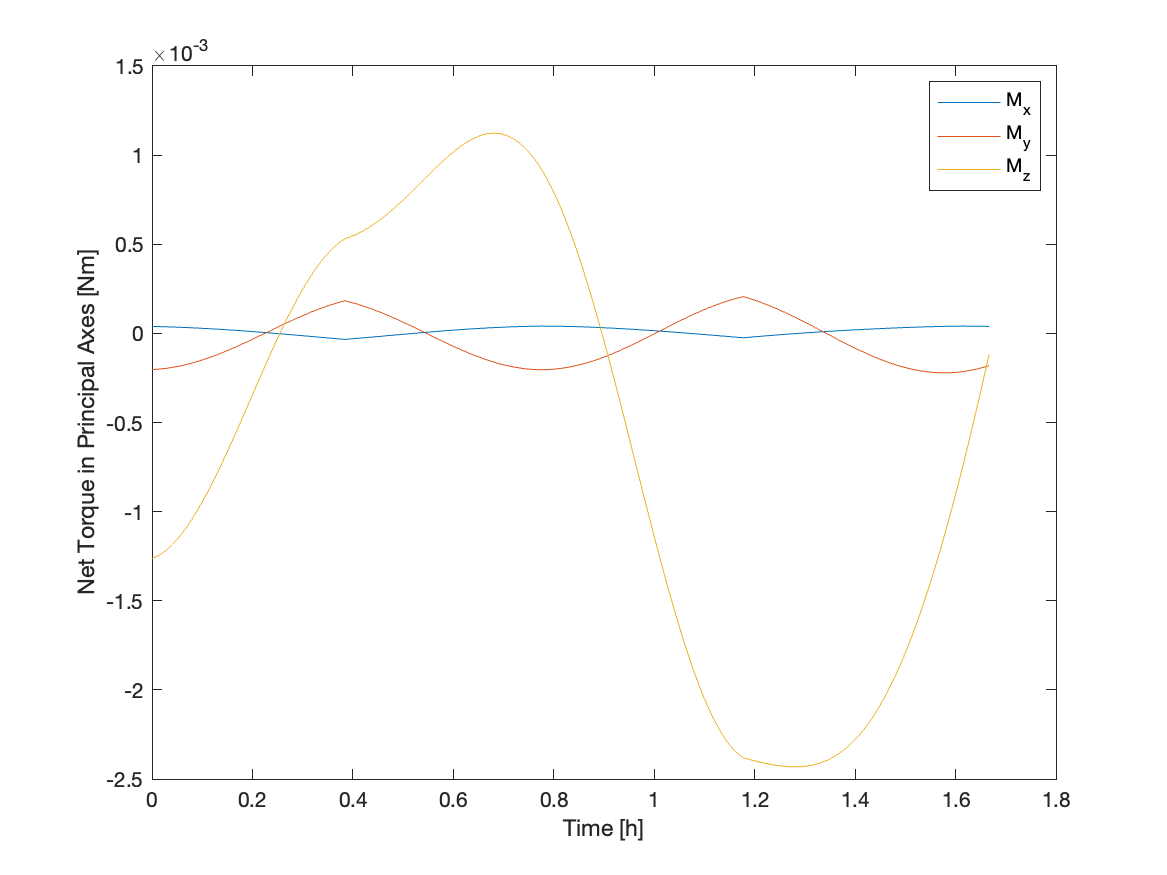
\includegraphics[scale=0.6]{Images/ps5_problem3_net.png}
\caption{Numerical simulation of net torques}
\label{fig:ps5_problem3_net}
\end{figure}